\documentclass{boi2014-pl}

\usepackage{enumitem}
\usepackage{todonotes}
\usepackage{wrapfig}

\renewcommand{\DayNum}{2}
\renewcommand{\TaskCode}{demarcation}
\renewcommand{\TaskName}{Demarkacja}
\renewcommand{\TaskVersion}{1.2}

\newcommand{\constant}[1]{{\tt #1}}

\begin{document}
    \begin{wrapfigure}{r}{3cm}
        \vspace{-24pt}
		\includegraphics[width=3cm]{\TaskCode.jpeg}
	\end{wrapfigure}

    Przez długie lata Bajtocja była wyspą, na której w pokoju żyli poddani króla Bajtazara I.
  Jednak po jego nagłej śmierci dwaj królewscy synowie -- bliźniacy Bitoni i Bajtoni -- nie
  mogli dojść do porozumienia, który z~nich powinien objąć tron. Postanowili więc podzielić
  wyspę na dwie prowincje, którymi będą rządzić niezależnie.

  Na prostokątnej mapie Bajtocja ma kształt wielokąta o $N$ wierzchołkach, przy czym każdy bok jest równoległy
  do jednego z~boków mapy, a każde dwa kolejne boki są prostopadłe.
  Żadne dwa boki nie dotykają się ani nie przecinają, oprócz kolejnych boków, które mają wspólny koniec.
  
  Bitoni i Bajtoni chcą podzielić ten wielokąt na dwie figury przystające za pomocą
  jednego odcinka równoległego do któregoś z boków mapy i zawartego w wielokącie.
  (Mówimy, że dwie figury są przystające, jeśli jedną z nich można przekształcić w drugą za pomocą symetrii, obrotów oraz przesunięć.)
  Zarówno współrzędne wierzchołków wielokąta, jak i końców odcinka dzielącego, są liczbami całkowitymi.

  Królewscy synowie poprosili Cię, abyś stwierdził, czy taki podział jest
  w ogóle możliwy.

    \Task

    Mając dany kształt wyspy, sprawdź, czy można ją podzielić za pomocą poziomego lub pionowego
    odcinka na dwa przystające wielokąty.
    Jeśli taki podział istnieje, znajdź dowolny odcinek, który go powoduje.

    \Input
	W pierwszym wierszu wejścia znajduje się jedna liczba całkowita $N$ -- liczba wierzchołków.
        $i$-ty z kolejnych $N$ wierszy zawiera parę liczb całkowitych $X_i$ oraz $Y_i$ ($0 \le X_i, Y_i \le 10^9$), oznaczających współrzędne $i$-tego wierzchołka.

        Wierzchołki są podane w kolejności ich występowania na obwodzie wielokąta,
        czyli odcinki $(X_1,Y_1) - (X_2,Y_2)$,
    $(X_2,Y_2) - (X_3,Y_3)$, \ldots, $(X_{N-1},Y_{N-1}) - (X_N,Y_N)$ oraz
    $(X_N,Y_N) - (X_1,Y_1)$ są kolejnymi bokami wielokąta.
        Ponadto, każde dwa kolejne boki są prostopadłe.

	\Output
        Twój program powinien wypisać jeden wiersz.
        Jeśli jest możliwy podział wyspy na dwa przystające wielokąty za pomocą poziomego lub pionowego odcinka o
        końcach w punktach $(x_1,y_1)$ oraz $(x_2,y_2)$, wypisz cztery liczby całkowite $x_1$, $y_1$, $x_2$, $y_2$ pooddzielane pojedynczymi odstępami.
        Musi zachodzić $x_1 = x_2$ lub $y_1 = y_2$.
        Odcinek musi w całości zawierać się wewnątrz danego wielokąta i tylko jego końce powinny dotykać brzegu wielokąta.
 
        Jeśli podział nie jest możliwy, wypisz pojedyncze słowo \constant{NO}.

    \clearpage

    \Examples
	\example
	{
		10 \newline
		0 0 \newline
		1 0 \newline
		1 1 \newline
		3 1 \newline
		3 5 \newline
		2 5 \newline
		2 3 \newline
		1 3 \newline
		1 2 \newline
		0 2
	}
	{
		1 2 3 2
	}
	{
        Poprawnym rozwiązaniem jest także\newline{\tt 3 2 1 2}.
	
        \begin{center}
            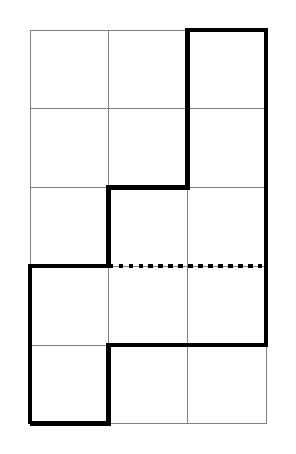
\begin{tikzpicture}
            \draw[help lines] (0,0) grid (3,5);
            \draw[ultra thick] (0,0) -- (1,0) -- (1,1) -- (3,1) -- (3,5) --
                         (2,5) -- (2,3) -- (1,3) -- (1,2) -- (0,2) -- (0,0);
            \draw[ultra thick,dotted] (1,2) -- (3,2);
            \end{tikzpicture}
        \end{center}
        }

	\example
	{
		6 \newline
		0 0 \newline
		1 0 \newline
		1 1 \newline
		2 1 \newline
		2 2 \newline
		0 2
	}
	{
		NO
	}
        {
        W tym przypadku nie da się podzielić wyspy na dwa przystające wielokąty.
        \begin{center}
            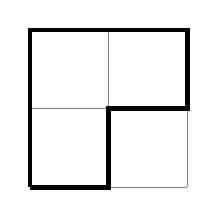
\begin{tikzpicture}
            \draw[help lines] (0,0) grid (2,2);
            \draw[ultra thick] (0,0) -- (1,0) -- (1,1) --
                         (2,1) -- (2,2) -- (0,2) -- (0,0);
            \end{tikzpicture}
        \end{center}
        }

    \Scoring

    \begin{description}
        \item[Podzadanie 1 (12 punktów).] $4 \le N \le 100\,000$.
        Każda prosta, która dzieli wielokąt na części, dzieli go na dokładnie dwie części.
        \item[Podzadanie 2 (15 punktów).] $4 \le N \le 200$
        \item[Podzadanie 3 (23 punkty).] $4 \le N \le 2\, 000$
        \item[Podzadanie 4 (50 punktów).] $4 \le N \le 100\, 000$
    \end{description}

    \Constraints

    \begin{description}
        \item[Limit czasu:] 0,5 s.
        \item[Dostępna pamięć:] 256 MB.
    \end{description}

\end{document}
